 \documentclass{beamer}

\usetheme{MagdeburgFIN}
\usefonttheme{structurebold}
\usepackage{graphicx}
\usepackage{float}
\usepackage{url}
\usepackage{pdfpages}


\title{Current state and future challenges in Optional Weaving}
\author{Constanze Michaelis}
\date{June 27, 2009}
\institute{Student Conference on Software Engineering and Database Systems}

\begin{document}

\begin{frame}[plain]
 \titlepage
\end{frame}



\section[Agenda]{}
\begin{frame}
\frametitle{Agenda}
\tableofcontents
\end{frame}

\section{Motivation}
\begin{frame}
\frametitle{Motivation}
\begin{itemize}
 \item software product lines at JETI
\begin{itemize}
	\item firmware was built according to pcb layout (spl with preprocessor)
	\item PC software was built ``new'' according to measurement device
	\item copy and paste including errors
	\item new errors emerging
	\item software was full of features $\Rightarrow$ one feature $\leftrightarrow$ one customer	
\end{itemize}
\end{itemize}
\end{frame}

\begin{frame}
\frametitle{Motivation}
\begin{itemize}
 \item software product lines (spl) become more and more important in software development
 \item major design principle of spl: separation of concerns 
 \item features 
	\begin{itemize}
	  \item describe concerns of spl
	  \item selectable units within spl
	  \item mandatory or optional
	\end{itemize}
 
\end{itemize}
\end{frame}

\begin{frame}
\frametitle{FOP/AOP}
\begin{itemize}
 \item separation of concerns realized with 
\begin{itemize}
\item aspect-oriented programming (AOP) 
\begin{itemize}
\item aims on separating the crosscutting concerns (code scattered across multiple components)
\item implementation of crosscutting concerns as aspects
\item pointcuts and advice for additional features, traditional design concepts for core
\end{itemize}
\end{itemize}
\begin{itemize}
\item feature-oriented programming (FOP)
\begin{itemize}
 \item aims on feature traceability
 \item idea: build program by composing features, where feature refines another feature incrementally
 \item features composed by mixin approach within AHEAD toolsuite
\end{itemize}
\end{itemize}
\end{itemize}
\end{frame}

\begin{frame}
\frametitle{FOP/AOP}
\begin{itemize}
 \item features in software product lines are often optional and interact with / depend on each other 
 \item leads to the feature optionality problem when features interact and are optional
 \item often interacting optional features were implemented mandatory 
\end{itemize}
\end{frame}
\section{Feature optionality problem}

\begin{frame}
\frametitle{Feature optionality problem}
\begin{center}
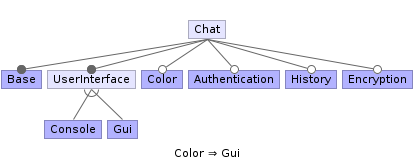
\includegraphics[width=.8\textwidth]{img/fm.png}
\end{center}
\pause
\begin{columns}
\column{.6\textwidth}
\begin{itemize}
 \item<1-> occurs when features that interact are optional 
 %\pause
\item<3-> first idea: encapsulation of interacting code as derivative feature 
\end{itemize}
\column{.4\textwidth}
\begin{center}
\begin{figure}
\includegraphics<1-2>[width=.6\textwidth]{img/fop.png}
\includegraphics<3>[width=.6\textwidth]{img/der.png}
\end{figure}
\end{center}
\end{columns}
\end{frame}

\section{Optional Weaving}

\begin{frame}
\begin{columns}
\column{.7\textwidth}
\frametitle{Optional Weaving}
\begin{itemize}
 \item implementation of optional interactions within feature
 \item i.e. the interaction code remains within feature but is optional 
 \item optional interaction code is woven when both features are implemented
\end{itemize}
\column{.3\textwidth}
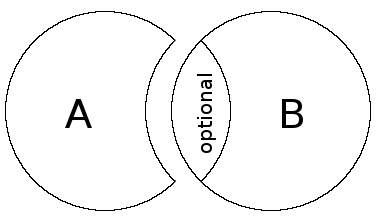
\includegraphics[width=.9\textwidth]{img/ow.png}
\end{columns}
\end{frame}

\begin{frame}
\frametitle{Optional Weaving}
\begin{itemize}
 \item FeatureC++
	\begin{itemize}
		\item combination of AOP and FOP 
		\item Approach:
		\begin{itemize}
		\item improvement of mixins to cope with optional features by introducing AOP concepts to mixins
		\item refinements with the keywords \emph{before, after, around} are optional
		\end{itemize}

	\end{itemize}
	\end{itemize}
\end{frame}

\begin{frame}
\frametitle{Optional Weaving}
\begin{itemize}
 \item AspectJ
	\begin{itemize}
		\item not usable for optional weaving in the current state because of
\begin{itemize}
 \item the lack of referencing optional classes, methods or member variables in optional advice statements resulting in code replication
\item this approach only for advice statements and not for inter type member declarations 
\end{itemize}
\pause
\item need to overcome these lacks because of
\begin{itemize}
 \item avoiding the need of creating derivative features
\item implementation of optional extension within the genuine feature $\Rightarrow$ maintain locally
\end{itemize}


	\end{itemize}
\end{itemize}
\end{frame}



\section{Conclusion}
\begin{frame}
\frametitle{Conclusion}
\begin{itemize}
 \item optional weaving is a promising approach 
 \begin{itemize}
  \item optionality is important for software product lines
  \item derivative approach will scale according to the derivatives
 \end{itemize}
 \item within FeatureC++ optional weaving implemented for two features 
 \item with AspectJ optional weaving leads to code replication and unnecessary code for runtime semantics
	 $\Rightarrow$improvements to the language must be made  
 
\end{itemize}
\end{frame}




\begin{frame}
 \frametitle{Thank you for your attention!}
\end{frame}


\end{document}
